\documentclass{report}
\usepackage[utf8]{inputenc}
\usepackage{hyperref}
\usepackage{graphicx}
\usepackage{amsmath}
\usepackage{amsfonts}
\usepackage{amssymb}
\usepackage{fancyhdr}
\usepackage{float}
\usepackage[backend=biber,style=alphabetic]{biblatex} % Ajout du package biblatex

\addbibresource{bibliographie.bib} % Spécifiez le fichier.bib contenant vos références

\title{Réseau et Sécurité - Rapport: Réseaux Privés Virtuels (VPN)}
\author{SANNA Thomas}
\date{\today}

\pagestyle{fancy}
\fancyhf{}
\fancyhead[L]{\leftmark}
\fancyhead[R]{\thepage}
\fancyfoot[R]{\thepage}
\fancyfoot[L]{Università di Corsica Pasquale Paoli}

\begin{document}

\maketitle

\begin{figure}
  \centering
  
\includegraphics[width=1\textwidth]{img/logouniv.png}
\end{figure}

\tableofcontents

\chapter{Introduction}
Un réseau privé virtuel (VPN) est une technologie qui permet d'établir une connexion sécurisée et chiffrée sur un réseau moins sécurisé, tel qu'Internet. Les VPN sont largement utilisés pour protéger la confidentialité des utilisateurs, sécuriser les communications et contourner les restrictions géographiques.

\begin{figure}[H]
  \centering
  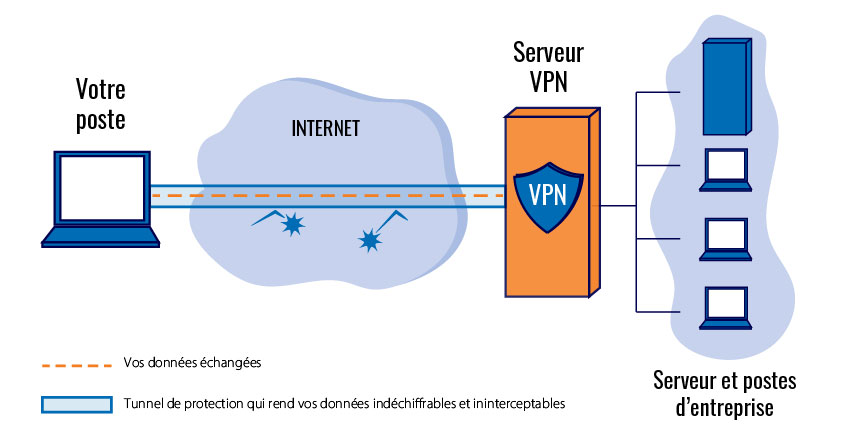
\includegraphics[width=1\textwidth]{img/schema-vpn-5.jpg}
  \caption{Illustration d'un VPN, source : \url{https://www.alliance-informatique.fr/wp-content/uploads/2022/06/schema-vpn-5.jpg}}
\end{figure}

\chapter{Fonctionnement d'un VPN}
\section{Architecture de base}
Un VPN fonctionne en créant un tunnel sécurisé entre l'appareil de l'utilisateur et un serveur VPN. Ce tunnel est chiffré, ce qui signifie que les données transmises sont illisibles pour quiconque intercepterait la communication.

\subsection{Attribution du VPN à l'utilisateur}
Pour attribuer un VPN à un utilisateur, celui-ci reçoit des informations de connexion, telles qu'un nom d'utilisateur, un mot de passe et parfois des certificats de sécurité. L'utilisateur configure ensuite son appareil (ordinateur, smartphone, etc.) avec ces informations pour établir une connexion sécurisée au serveur VPN. Le serveur VPN attribue une adresse IP virtuelle à l'utilisateur, masquant ainsi son adresse IP réelle et permettant de sécuriser ses communications.

\section{Types de VPN}
Il existe principalement trois types de VPN, chacun ayant des caractéristiques et des utilisations spécifiques \cite{2} :

\subsection{VPN client-to-site}
Le VPN client-to-site, également connu sous le nom de VPN d'accès à distance, permet à un utilisateur individuel de se connecter à un réseau privé à distance. Ce type de VPN est couramment utilisé par les employés pour accéder aux ressources de l'entreprise depuis leur domicile ou lors de déplacements. Le client VPN installé sur l'appareil de l'utilisateur établit une connexion sécurisée avec le serveur VPN de l'entreprise.

\begin{figure}[H]
  \centering
  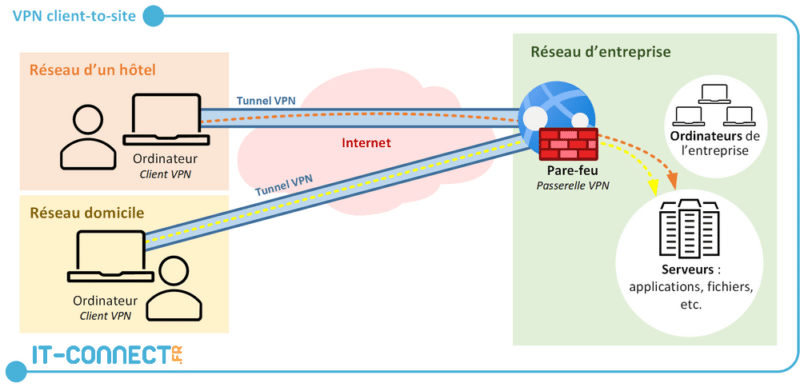
\includegraphics[width=1\textwidth]{img/clientToSite.png}
  \caption{Illustration d'une architecture Client-to-Site, source : \url{https://www.it-connect.fr/les-tunnels-vpn-pour-les-debutants}}
\end{figure}

\subsection{VPN site-to-site}
Le VPN site-to-site connecte deux réseaux locaux (LAN) distincts sur Internet, permettant aux utilisateurs de chaque réseau de communiquer comme s'ils étaient sur le même réseau local. Ce type de VPN est souvent utilisé pour relier les bureaux distants d'une entreprise, facilitant ainsi le partage de ressources et la collaboration entre les sites.

\begin{figure}[H]
  \centering
  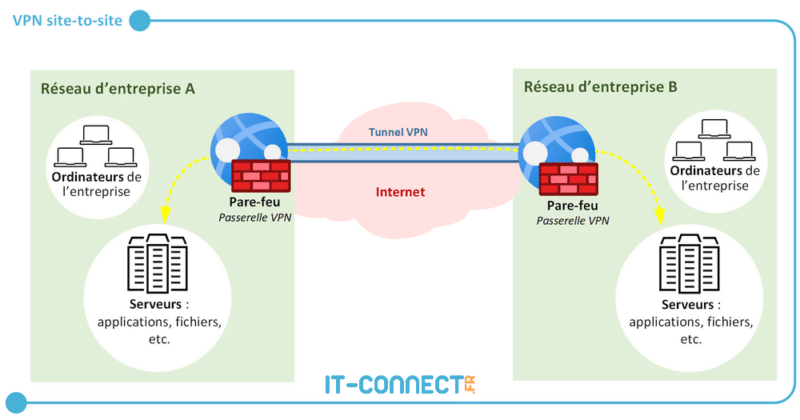
\includegraphics[width=1\textwidth]{img/siteToSite.png}
  \caption{Illustration d'une architecture Site-to-Site, source : \url{https://www.it-connect.fr/les-tunnels-vpn-pour-les-debutants}}
\end{figure}

\subsection{VPN grand public}
Le VPN grand public, ou VPN commercial, est destiné aux utilisateurs individuels qui souhaitent protéger leur vie privée en ligne et contourner les restrictions géographiques. Ces VPN sont fournis par des services VPN commerciaux et permettent aux utilisateurs de se connecter à des serveurs situés dans différents pays, masquant ainsi leur adresse IP réelle et chiffrant leur trafic Internet.

\begin{figure}[H]
  \centering
  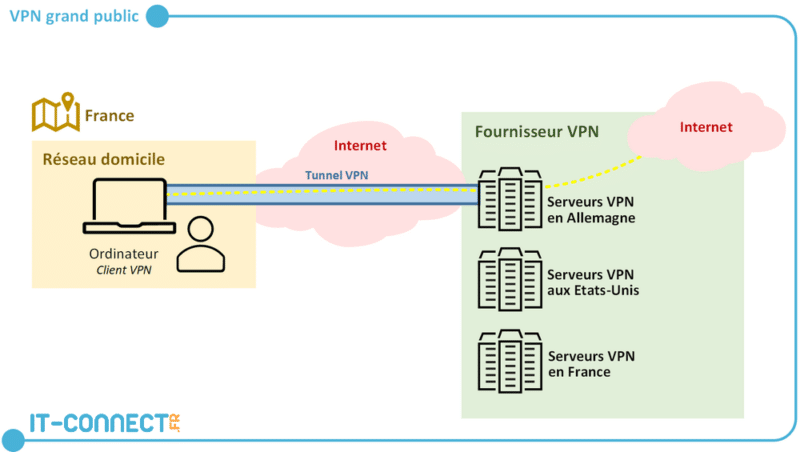
\includegraphics[width=1\textwidth]{img/grandPublic.png}
  \caption{Illustration d'une architecture Grand Public, source : \url{https://www.it-connect.fr/les-tunnels-vpn-pour-les-debutants}}
\end{figure}

\section{Protocoles VPN}
Les VPN utilisent divers protocoles pour établir et sécuriser les connexions. Ces protocoles sécurisent principalement les connexions entre l'utilisateur et le serveur VPN. Une fois que les données atteignent le serveur VPN, elles sont transmises sur Internet de manière sécurisée, mais la protection dépend également des protocoles utilisés par les services finaux. Parmi les plus courants, on trouve :

\begin{itemize}
  \item \textbf{PPTP (Point-to-Point Tunneling Protocol)} : Un des plus anciens protocoles VPN, facile à configurer mais considéré comme moins sécurisé. Il utilise le protocole GRE (Generic Routing Encapsulation) pour encapsuler les paquets de données. Bien que rapide, il présente des vulnérabilités connues et est généralement déconseillé pour les applications nécessitant une sécurité élevée.
  \item \textbf{L2TP/IPsec (Layer 2 Tunneling Protocol)} : Combine L2TP avec le protocole de sécurité IPsec pour offrir une sécurité renforcée. L2TP crée le tunnel et IPsec assure le chiffrement des données. Ce protocole est plus sécurisé que PPTP, mais peut être plus lent en raison du double encapsulage des données.
  \item \textbf{OpenVPN} : Un protocole open-source très sécurisé et flexible, utilisant SSL/TLS pour le chiffrement. OpenVPN peut fonctionner sur n'importe quel port, ce qui le rend difficile à bloquer par les pare-feu. Il est considéré comme l'un des protocoles VPN les plus sécurisés et est largement utilisé par les services VPN commerciaux.
  \item \textbf{IKEv2/IPsec (Internet Key Exchange version 2)} : Offre une connexion rapide et stable, particulièrement utile pour les appareils mobiles. IKEv2 est connu pour sa capacité à rétablir rapidement les connexions après une interruption, ce qui le rend idéal pour les utilisateurs mobiles qui passent fréquemment d'un réseau à un autre.
  \item \textbf{WireGuard} : Un protocole VPN relativement nouveau qui promet des performances élevées et une sécurité robuste. WireGuard utilise des algorithmes de cryptographie modernes et est conçu pour être plus simple et plus rapide que les protocoles VPN traditionnels. Il est de plus en plus adopté par les services VPN en raison de son efficacité et de sa facilité de déploiement.
\end{itemize}

\begin{figure}[H]
  \centering
  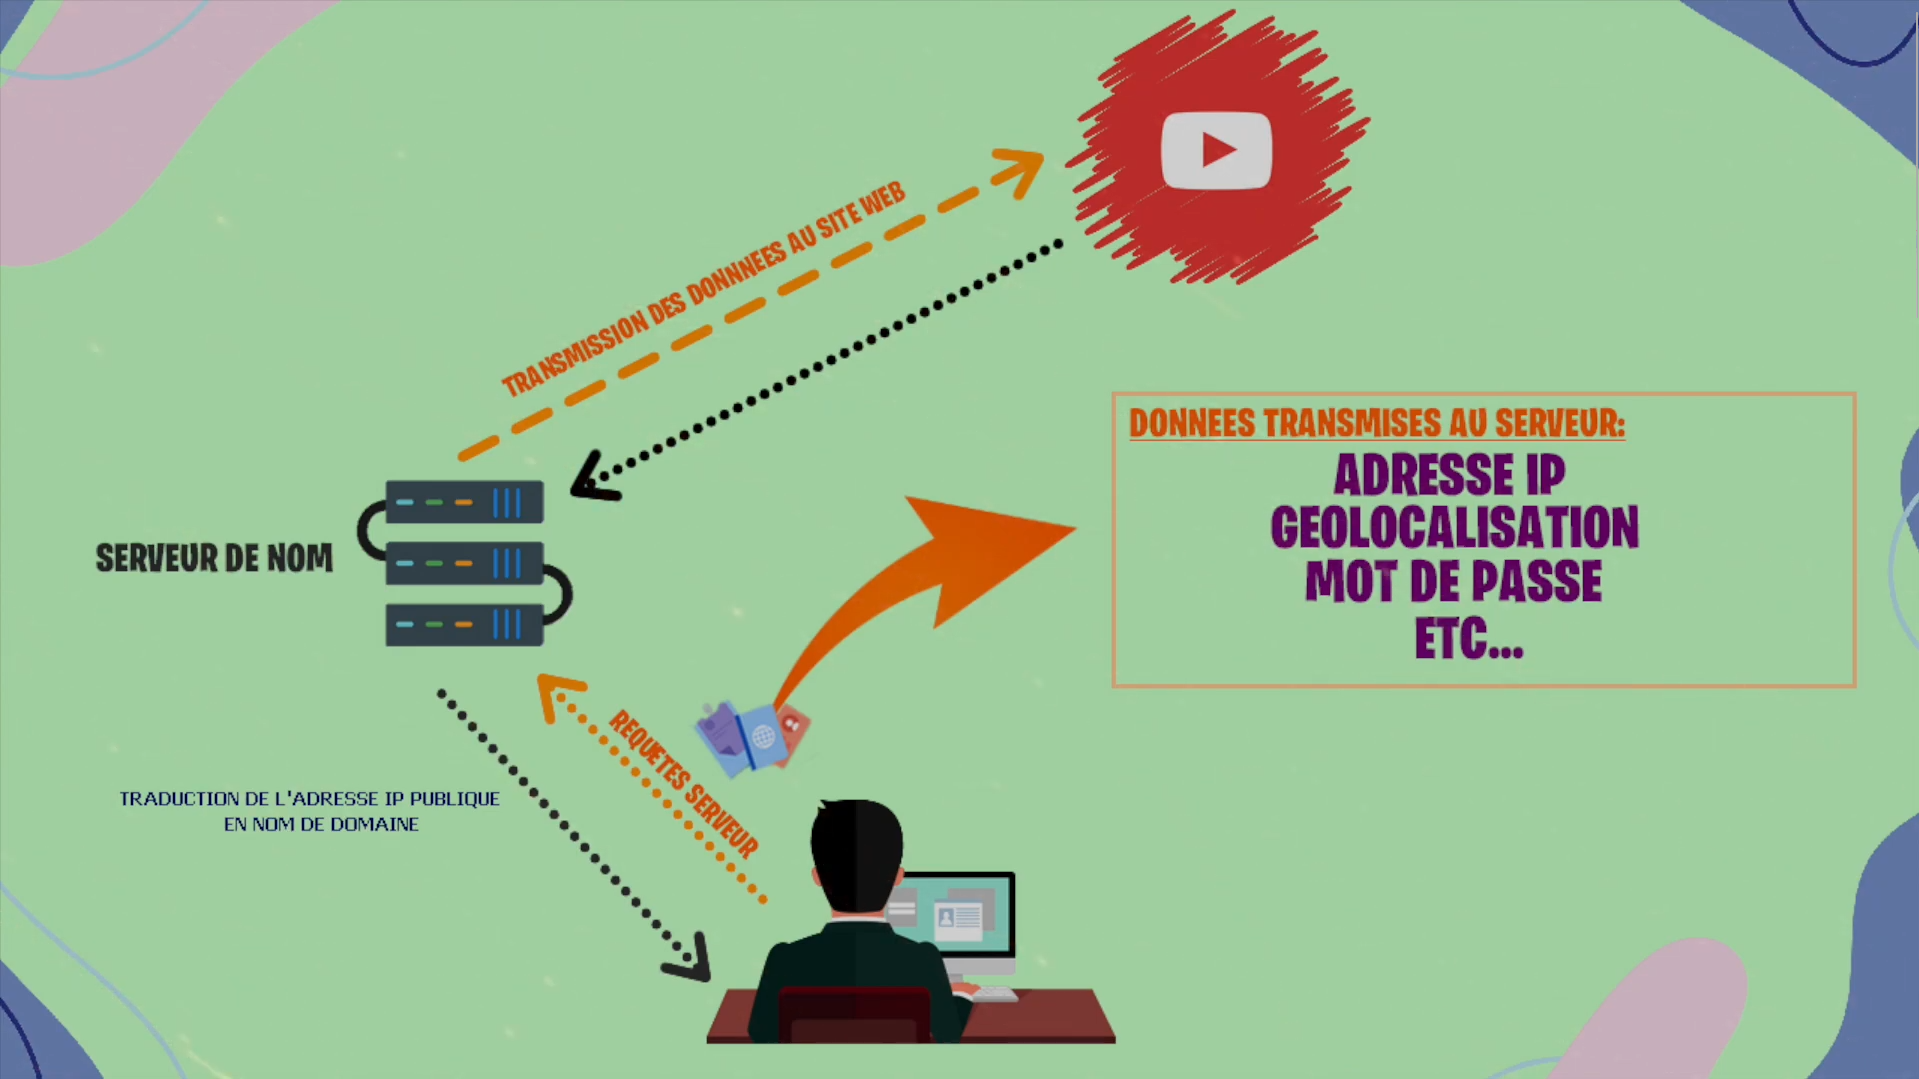
\includegraphics[width=1\textwidth]{img/novpn.png}
  \caption{Illustration de la navigation sans VPN, source : \url{https://www.youtube.com/watch?app=desktop&v=IWss3sGV4mI}}
\end{figure}

\begin{figure}[H]
  \centering
  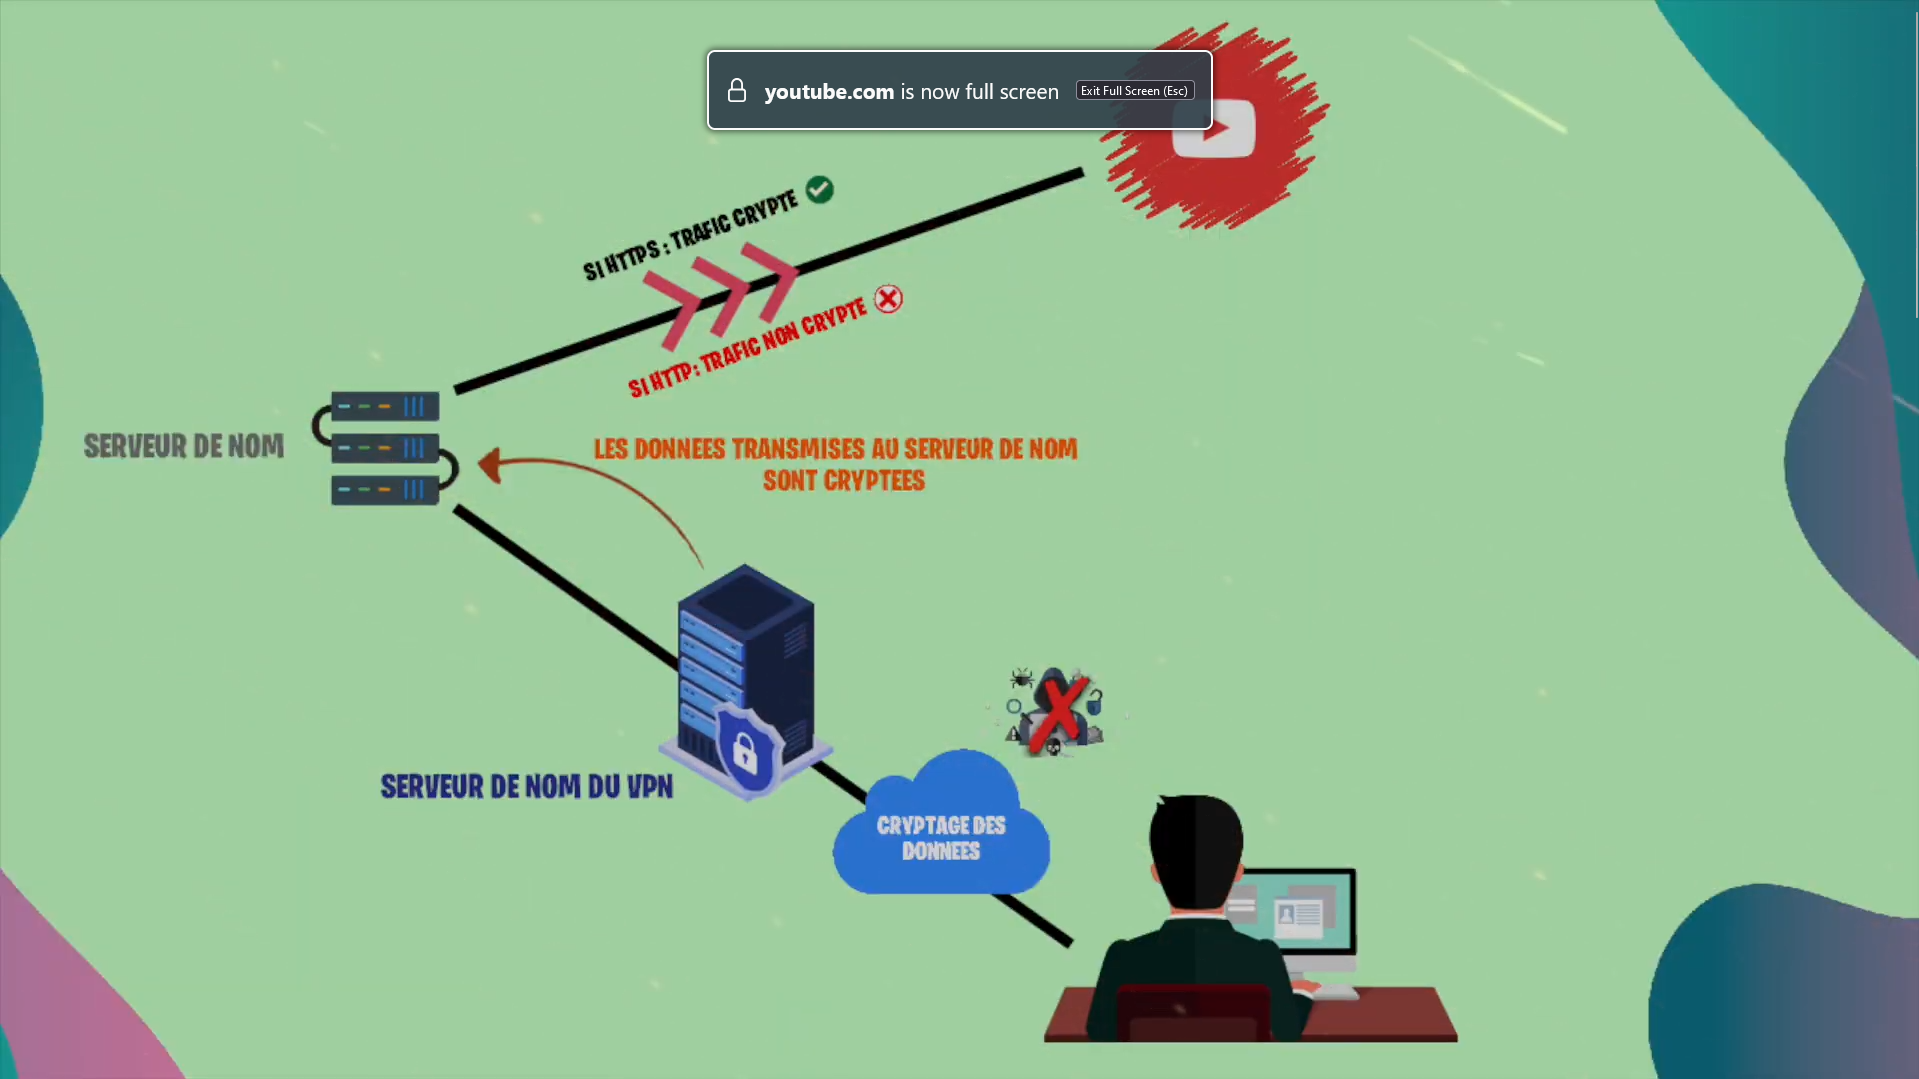
\includegraphics[width=1\textwidth]{img/vpn.png}
  \caption{Illustration du chiffrement VPN, source : \url{https://www.youtube.com/watch?app=desktop&v=IWss3sGV4mI}}
\end{figure}

\break\section{Chiffrement}
Le chiffrement est une composante essentielle des VPN. Il transforme les données en un format illisible sans la clé de déchiffrement appropriée. Les algorithmes de chiffrement couramment utilisés incluent AES (Advanced Encryption Standard) et RSA (Rivest-Shamir-Adleman). AES est souvent utilisé en raison de sa rapidité et de sa sécurité, tandis que RSA est utilisé pour l'échange de clés sécurisées.

\section{Création d'un Tunnel VPN}
Le processus général de création d’un tunnel VPN est le suivant \cite{1} :

\begin{itemize}
  \item \textbf{Encapsulation} : Les méthodes d’encapsulation courantes comprennent le protocole IP-in-IP et l’encapsulation générique de routage (GRE).
  \item \textbf{Interface réseau virtuelle} : Crée un adaptateur réseau virtuel sur le périphérique client, servant de point d’extrémité du tunnel.
  \item \textbf{Établissement d’un canal sécurisé} : Établit un canal de communication chiffré à l’aide d’algorithmes et de clés négociés. (Avec des protocoles tels que SSL/TLS, IPsec, etc.)
  \item \textbf{Test du tunnel} : Peut envoyer un paquet de test pour vérifier qu’il fonctionne correctement.
  \item \textbf{Mécanismes de maintien en vie} : Établit des protocoles pour maintenir le tunnel, en évitant les dépassements de délai de connexion.
  \item \textbf{Paramètres de qualité de service (QoS)} : Configure les paramètres pour gérer les priorités du trafic dans le tunnel.
\end{itemize}

Ce processus garantit que les communications entre l'utilisateur et le serveur VPN sont sécurisées et protégées contre les interceptions et les attaques.


\chapter{Anonymisation et Confidentialité}
\section{Masquage de l'adresse IP}
L'une des principales raisons pour lesquelles les utilisateurs choisissent d'utiliser un VPN est de masquer leur adresse IP réelle. En se connectant à un serveur VPN, l'adresse IP visible par les sites web et services en ligne est celle du serveur VPN, et non celle de l'utilisateur.

\section{Protection contre la surveillance}
Les VPN protègent également contre la surveillance en chiffrant les données. Cela empêche les FAI (fournisseurs d'accès à Internet), les gouvernements et les pirates informatiques de surveiller les activités en ligne de l'utilisateur.

\break\section{Contournement des restrictions géographiques}
Les VPN permettent de contourner les restrictions géographiques en faisant apparaître l'utilisateur comme s'il se connectait depuis un autre emplacement. Cela est particulièrement utile pour accéder à des contenus restreints ou censurés dans certaines régions.

\begin{figure}[H]
  \centering
  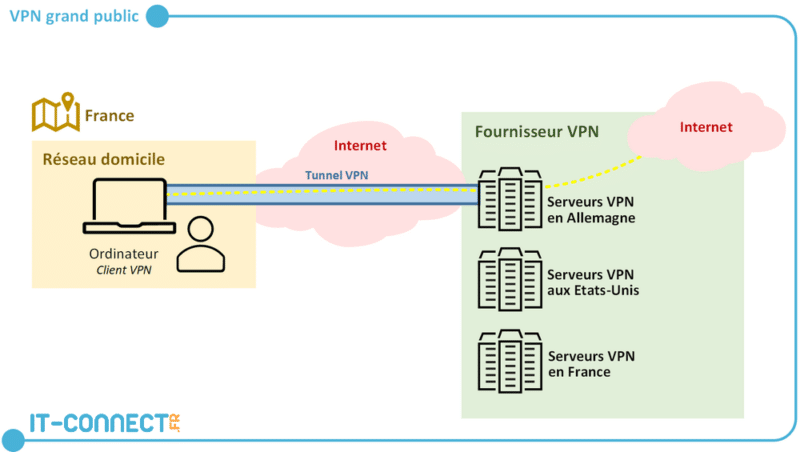
\includegraphics[width=1\textwidth]{img/localisation.png}
  \caption{Illustation de plusieurs serveurs situés aux quatres coins du monde, source : \url{https://www.it-connect.fr/les-tunnels-vpn-pour-les-debutants/}}
\end{figure}

\chapter{Sécurité des Réseaux et VPN}
\section{Menaces et Attaques}
Les réseaux sont constamment menacés par diverses attaques, telles que les attaques par déni de service (DoS), les attaques de l'homme du milieu (MitM), et les intrusions non autorisées. Les VPN aident à atténuer ces menaces en sécurisant les communications.

\section{Meilleures Pratiques}
Pour maximiser la sécurité lors de l'utilisation d'un VPN, il est recommandé de :
\begin{itemize}
  \item Utiliser des protocoles de chiffrement forts.
  \item Choisir des fournisseurs VPN réputés qui ne conservent pas de journaux d'activité.
  \item Mettre régulièrement à jour les logiciels VPN pour bénéficier des dernières améliorations de sécurité.
\end{itemize}

\chapter{Conclusion}
Les VPN sont des outils puissants pour protéger la confidentialité et la sécurité en ligne. En chiffrant les communications et en masquant l'adresse IP de l'utilisateur, ils offrent une couche supplémentaire de protection contre la surveillance et les attaques. Cependant, il est crucial de choisir un service VPN fiable et de suivre les meilleures pratiques pour garantir une sécurité optimale.

\printbibliography % Affiche la bibliographie

\end{document}